\documentclass[ letterpaper,12pt]{article}

\usepackage[english]{babel}
\usepackage[T1]{fontenc}
\usepackage{a4wide}
\usepackage{graphicx}
%\usepackage{pngfig}

\begin{document}

\title{\textbf{DccNiTghtmare User's Documentation - 0.2}}

\author{
DNTeam
}

\maketitle

\abstract{This document is the User's manual of the DccNiTghtmare Game.}

\newpage

\tableofcontents

\newpage

\section{Introduction}

Welcome to the user's manual of DccNiTghtmare. Here you'll find all the
DccNiTghtmare's computer game related things that you need to know to play
DccNiTghtmare on your machine. 

\section{Compiling}

\subsection{Requeriments}

The compilation and execution of DccNiTghtmare requires the follow librarys and hardware:

\subsubsection{Software}
\begin{itemize}
\item{OpenGL (and the OpenGL drivers for your videocard)}
\item{SDL - Version 1.2.13, www.libsdl.org}
\item{SDL\_image - Version 1.2.6, www.libsdl.org/projects/SDL\_image}
\item{SDL\_ttf - Version 2.0.9, http://www.libsdl.org/projects/SDL\_ttf}
\item{OpenAL - Version 0.0.8, www.openal.org }
\item{Cal3D - Version 0.11, http://cal3d.sf.net}
\item{libogg - Version 1.1.3, http://xiph.org/ogg/}
\item{libvorbis - Version 1.2.1, http://xiph.org/vorbis}
\end{itemize}

\subsubsection{Hardware}
A video card with 3d aceleration enabled in Linux, compatible with OpenGL
(something better than a Geforce 6200 is recommended).

\subsection{Process}

Untar the bzip2 ball with command "tar -xvjf dccnitghtmare-src-02.tar.bz2";\\
Go to the dccnitghtmare folder with "cd dccnitghtmare";\\
Execute the command "make" to make the source code.

\section{Executing Without Installing}

To run DccNiTghtmare, go to the subfolder bin, in the directory dccnitghtmare, and run the dccnitghtmare binary:\\
" cd dccnitghtmare/bin "\\
" ./dccnitghtmare "

\section{Installing}

Just do a make install at dccnitghtmare folder, as root.

\subsection{Main Menu}

The main menu window appears on the screen, looking like the bellow {\it figure}. There are five buttons, and the title of the window describes the dccnitghtmare's version.

\begin{center}
  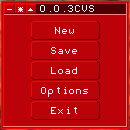
\includegraphics{mainMenuWindow.png}
\\{\bf Figure} - Main Menu Window
\end{center}

The options to choose are:

\begin{itemize}
\item{{\it New Game} - To start a new game with a new character;}
\item{{\it Continue} - To return to the current game ({\it if in game});}
\item{{\it Load} - To load an existent game; {\bf Not yet implemented!}}
\item{{\it Save} - To save the current game ({\it if in game}); {\bf Not yet implemented!}}
\item{{\it Options} - To manipulate the game options;}
\item{{\it Exit} - To exit the game;}
\end{itemize}

\subsection{Options}

In the options window you can change music and sound effects volume ( == 0
means no sound or no music) and change the main language of the game. For now
we offer full support to Portuguese and English languages and partial support
to French and Spanish.

\begin{center}
  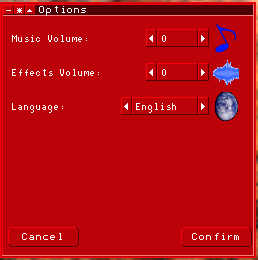
\includegraphics{optionsWindow.png}
\\{\bf Figure} - Options Window
\end{center}

Also, you can change the camera mode, to the Driven Camera, where the camera
follows the character orientation, or the Normal Camera Mode. You can, too,
enable/disable the particle system effects and the grass effects (the grass
effect will only be avaible if the particle system is).

\section{Creating Character}

Since DccNiTghtmare is a rpg D\&D friendly game, the player have to create a
character to play, with unique stats. All things that a player character can be
are described in the DccNiTghtmare Player's Book, avaible at
http://dccnitghtmare.sf.net .

All rpg rules are D\&D like, so if you played the D\&D somewhere you'll easy
understand all character's things here.

\subsection{Race}

\begin{center}
%\includegraphics{raceWindow.png}\\
{\bf Figure} - Race Window
\end{center}

In the race window you select the race of your character. The race affects how
well your character can do on each class. Your character race gives you plenty
of cues to what sort of person it is, the reactions to others races and some
special abilities they can have.

Just select the race you want to your character and click in the "Confirm"
button.

\subsection{Class}

Students seek gold, glory, revolution, knowledge, tecnology, scores, or maybe
some other goal - perhaps noble or perhaps base. Each chooses a different way
to attain those goals, from brutal Maths Power to a mighty Biology Creature, to
subtle skills. Some students can end their course. Others die trying to take
the diploma.

Your character class is its desired Career. Choose them carefully, since each
of them have distinct abilities.

\begin{center}
%%  \includegraphics{classWindow.png}
{\bf Figure} - Class Window
\end{center}


\subsection{Alignment \& Tendency}

Just choose the "Software-License-Thought-Like" your character have at the
Alignment \& Tendency window.

\begin{center}
%%  \includegraphics{alignWindow.png}
{\bf Figure} - Alignment \& Tendency Window
\end{center}

\subsection{Gender}

The gender is the sex tendency of your character.

{\bf WINDOW NOT YET IMPLEMENTED}

\subsection{Attributes}

\begin{center}
  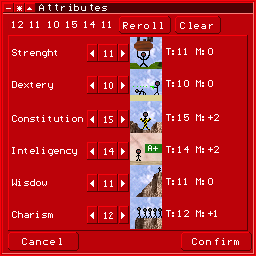
\includegraphics{attWindow.png}
\\{\bf Figure} - Attributes Window
\end{center}

In the attributes window you have to Roll Dices to determine each character's
atributes. Entering on the window, the dices were throwed to you: if you
dislike the values, just hit the button "Roll".  After having the desired
values, just assign each of them to some attribute (clicking on > or < button
of the desired attribute). 

To clear all assign attributes, just hit the button "Clear" and start the
assignment again. After define all attributes, just hit the button "Confirm".

\subsection{Skills}

\begin{center}
  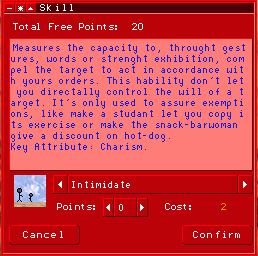
\includegraphics{skillWindow.png}
\\{\bf Figure} - Skills Window
\end{center}

In the skills window, you can redistribute all your avaible points to the skills you want. The cost of each skill means how many free points you'll need to increase one point in the skill.

The number of avaible skill points vary based on character's class and race, and also, level.

\subsection{Feats}

{\bf WINDOW NOT YET IMPLEMENTED}

\section{In-Game}

The main game window is composed by 2 basic windows, the visualization of the world and the player's portrait. Bellow we'll describe them.

\begin{center}
  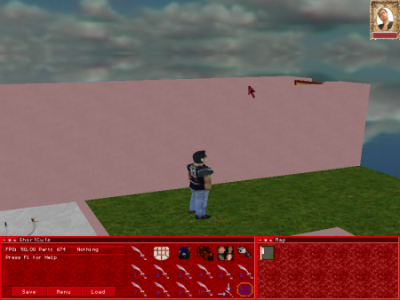
\includegraphics{mainGame.png}
\\{\bf Figure} - Main Game Window
\end{center}

\subsection{ShortCuts Window}

\begin{center}
  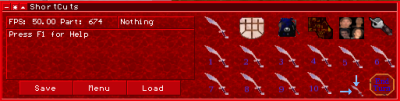
\includegraphics{shortcutsWindow.png}
\\{\bf Figure} - ShortCuts Window
\end{center}

The ShortCuts window is used to give the user many informations of things
current occurring on game and, also, to take from them some basic actions.

The window is composed, on the left corner, from 3 text boxes: the upper left
one, shows the current FPS of the game and the actual number of particles in
map; the upper right one, describes the name of the object or reactor pointed
by user's mouse; the last one shows informations about the fight, if in fight
mode, or about some done action.

Also, in the left corner, three shortcut buttons exists. One to load an saved
game ({\it the load function is not yet implemented}), other to go to the main
game menu, and the last to save the game ({\it the save function is not yet
implemented}).

On the right corner, there are 18 shortcuts buttons. From left to right they
are, on the first row: Button to enter the attack mode (with surprise attack to
the player character), to enter the defend mode, to open the player's
inventory, to open the map window, to open the party window, to view the player
character's informations. On the second row, the first six shortcuts to
assigned attacks. On the third row, the last four shortcuts to assigned
attacks, the button to open the assign attacks window and the button to end the
player character's turn.

This window can be opened by the keyboard 'n' key.

\subsection{Map Window}

\begin{center}
  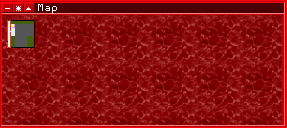
\includegraphics{mapWindow.png}
\\{\bf Figure} - Map Window
\end{center}

The map window represents the actual world map that is open. Also, the yellow square represents the current player character's position on the map. 

This window can be opened by the keyboard 'm' key, or by the map button on ShortCuts window.

\subsection{Character's Portrait}

\begin{center}
  
\includegraphics{portrait.png}
\\{\bf Figure} - Character's Portrait
\end{center}

The character's portrait represents the active player character, and his health status. There are a health bar (in red), showing how much of the total life points actual left.

\subsection{Commands}

\begin{tabular}{|c|c|}
\hline
F1 & Open quick help screen\\
\hline
Esc & Go To Main Menu\\
\hline
0-9 & Shortcut to assigned attacks\\
\hline
r & Show Character's Range of Action\\
\hline
space & Enter Battle Mode\\
\hline
y & Demonstrate Protect Effect\\
o & Demonstrate Blood Effect\\
p & Demonstrate Blood Effect\\
\hline
Right Mouse Click & Walk character to position\\
Left Mouse Click & Do Action on position\\
Middle Button Click & Rotate the Screen on mouse move\\
\hline
a & Turn Left\\
d & Turn Right\\
w & Step Forward\\
s & Step Backward\\
q & Step Left\\
e & Step Right\\
\hline
Left Arrow & Turn Camera Left\\
Right Arrow & Turn Camera Right\\
Up Arrow & Increases Zoom\\
Down Arrow & Decreases Zoom\\
Home & Maximize Zoom\\
End & Minimize Zoom\\
PageUp & Move Camera Up\\
PageDown & Move Camera Down\\
Insert & Move Camera to Top\\
Delete & Move Camera to Floor\\
\hline
\end{tabular}

\subsection{Icons Actions}

\begin{tabular}{|c|c|}
\hline
 
\includegraphics{Get.png} & Get, if posible, an object\\
\hline
 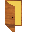
\includegraphics{Door.png} & Open, if possible, a door\\
\hline
 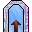
\includegraphics{MapTravel.png} & Travel to another map\\
\hline
 
\includegraphics{Walk.png} & Walk with the character to some map point\\
\hline
 
\includegraphics{talk.png} & In normal mode, talk to a character\\
\hline
 
\includegraphics{Attack.png} & If in attack mode, attack a character\\
\hline
\end{tabular}

\subsection{Fighting}

The fighting mode is, in somethings, distinct than the normal mode of the game.
Here the character's movimentation is limited and their action is taken in
turns.

The game went to fight mode when there are enemies in range area or you want to attack any NPC in the area.

\subsubsection{Initing a Fight}

When you want to init by yourself the fight mode, you can use the button of fight in the ShortCuts Window. By done it, you enter in the fight mode, in your active character's turn (called surprise attack turn) where functions like any other normal turn. If at the end of this turn you've not attacked, the game exits the attack mode. Otherwise, continue the fight in the  correspondent initiative values orderf.

\subsubsection{Player Character's Turn}

\begin{center}
  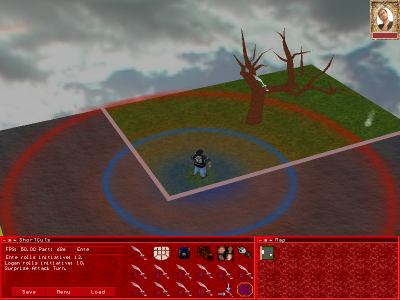
\includegraphics{fightMode.png}
\\{\bf Figure} - Fight Mode
\end{center}

When is player character's turn, like D\&D, the character can take a standart action and a move action, in any order, two move actions or a full round action. The area that the character can walk with one move action is represented in the blue circle; the two move actions is represented in the red circle.

The player choose the actions to be made on the turn, doing all of them and, when done with it, end the turn.

\subsubsection{End Turn}

When you done all things that you want (and that you can) in your turn, you can pass the fight to next character's turn. You can do it by clicking in the ShortCuts Window button of End Turn.

\subsection{Talking}

To talk to a NPC you need to be on normal game mode, put your mouse cursor in
the target NPC, showing the talk mouse cursor 
\includegraphics{talk.png},
and press the left mouse button.

The talk window will open, showing the things npc talked and the options your character can talk to him. You need do be in range to can talk, with your character get out of range, the conversation will be stop, like you abandoned it.

{\bf NOT YET IMPLEMENTED!}

\subsection{Inventory}

{\bf NOT YET IMPLEMENTED!}

\subsection{Sugestions and Help}

We are an open group, if you have some sugestions to to DccNiTghtmare or want to help the development of the game in some manners, just contact us at sourceforge.

\end{document}

